%!TEX root=../main.tex
\section{Application} % (fold)
\label{sec:application}

\textcolor{red}{We implement our methodology utilizing data from the National Basketball Association (NBA). To access comprehensive game data, we utilize the Python package \texttt{nba\_api}\footnote{\url{https://github.com/swar/nba_api/}}, which provides access to the APIs of \url{nba.com}. The dataset encompasses shot location data from all NBA games spanning the seasons between $2018-2019$ and $2022-2023$. Filtering the dataset, we focus solely on players who have made more than $1000$ shots during this five-season period, resulting in a cohort of $131$ players. These players accounted for a total of $493723$ shots attempted, of which $234941$ were successful. Subsequently, we exclude shots deemed impossible (e.g., out-of-bounds), leaving us with a dataset comprising $492621$ shots. To analyze shooting behavior, we employ 2-dimensional kernel density estimation, utilizing Silverman's rule \citep{silvermanDensityEstimationStatistics1986} for bandwidth estimation. The density estimation is conducted on a regularly spaced grid consisting of $51 \times 51$ points.}

\begin{figure}
    \centering
    \begin{subfigure}[b]{0.49\textwidth}
        \centering
        \includegraphics[width=\textwidth]{figures/curry_make_miss.pdf}
        \caption{Stephen Curry}
        \label{fig:curry_make_miss}
    \end{subfigure}
    \hfill
    \begin{subfigure}[b]{0.49\textwidth}
        \centering
        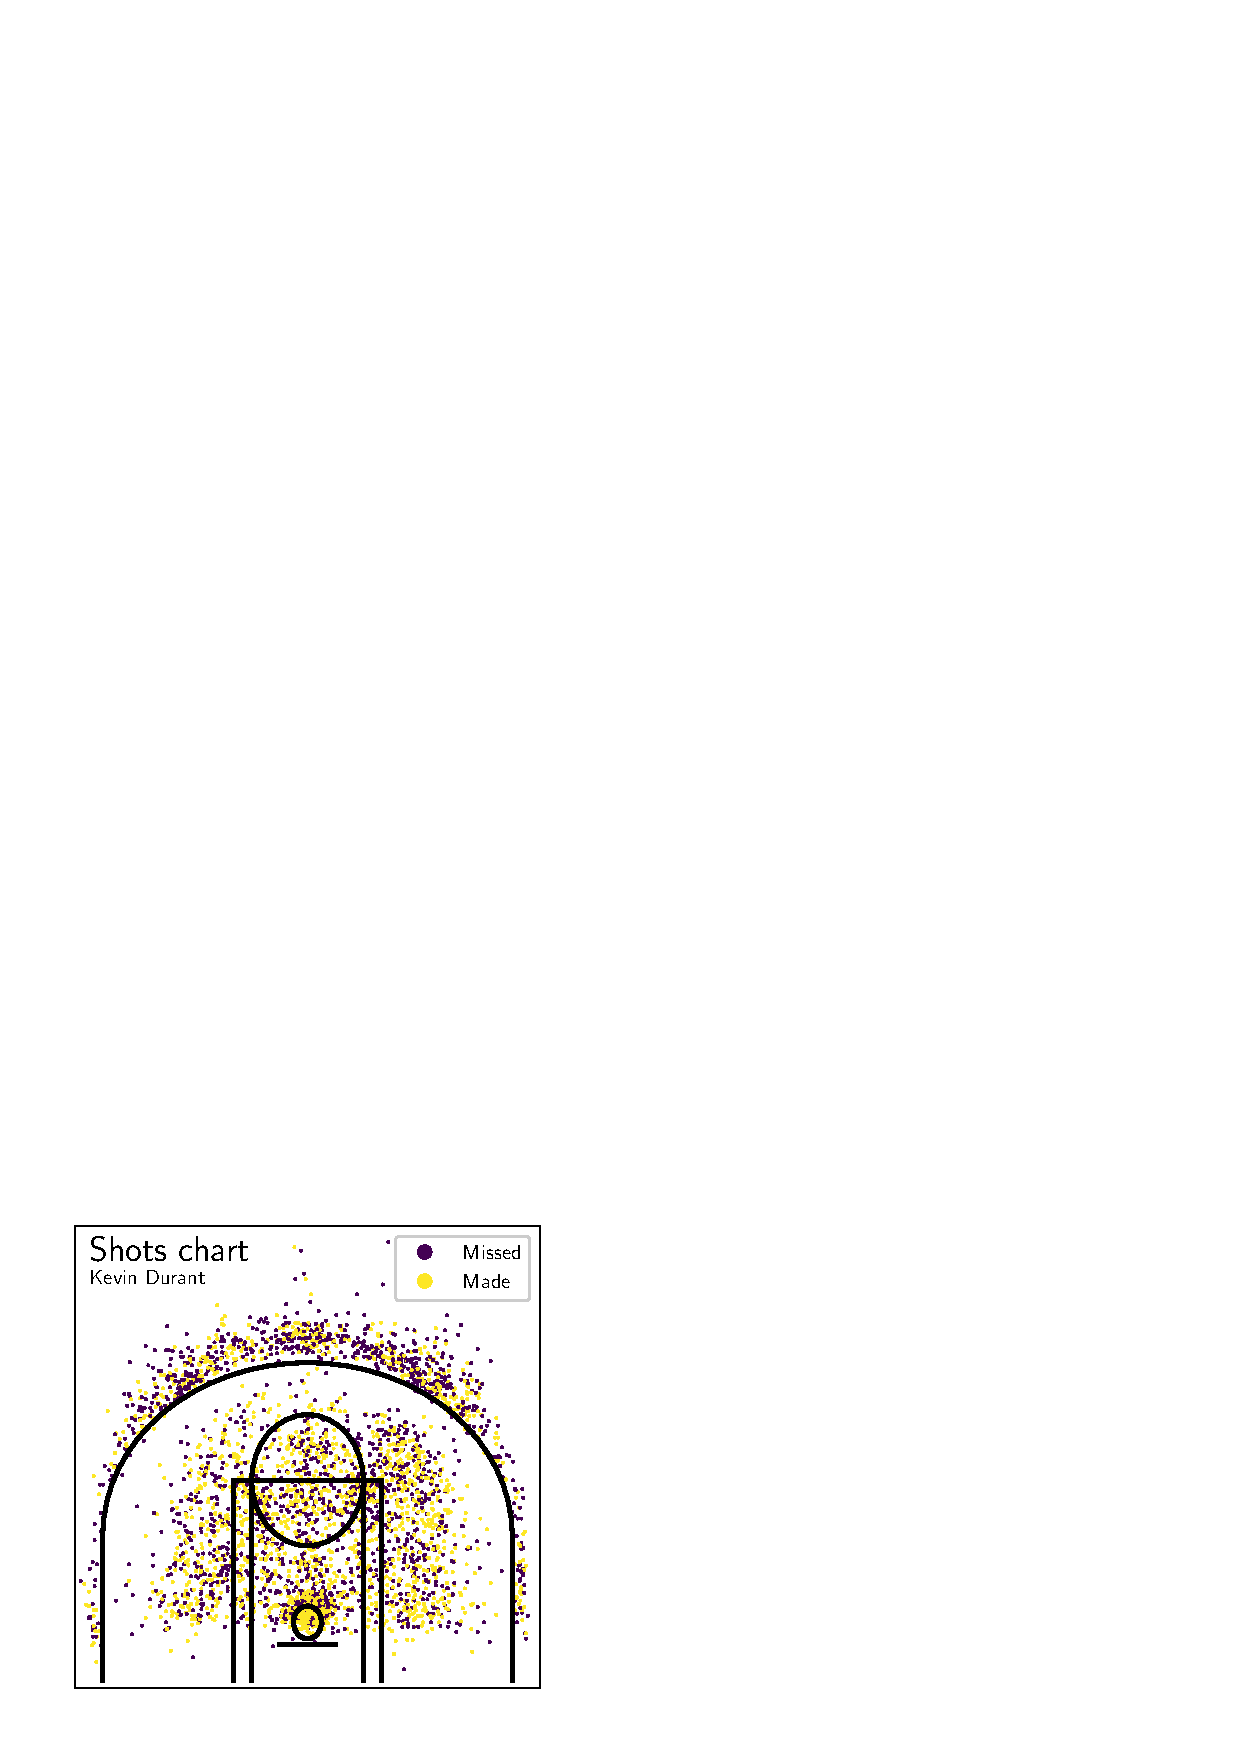
\includegraphics[width=\textwidth]{figures/durant_make_miss.pdf}
        \caption{Kevin Durant}
        \label{fig:durant_make_miss}
    \end{subfigure}
    \caption{Make/Miss chart for Stephen Curry and Kevin Durant.}
    \label{fig:shoots_make_miss}
\end{figure}


\textcolor{red}{A MFPCA is run on the data. Figure \ref{fig:curry_shoots_decomposition} shows examples of the shooting densities of Stephen Curry and their first five functional principal components.}
\begin{figure}
    \centering
    \begin{subfigure}[b]{0.45\textwidth}
        \centering
        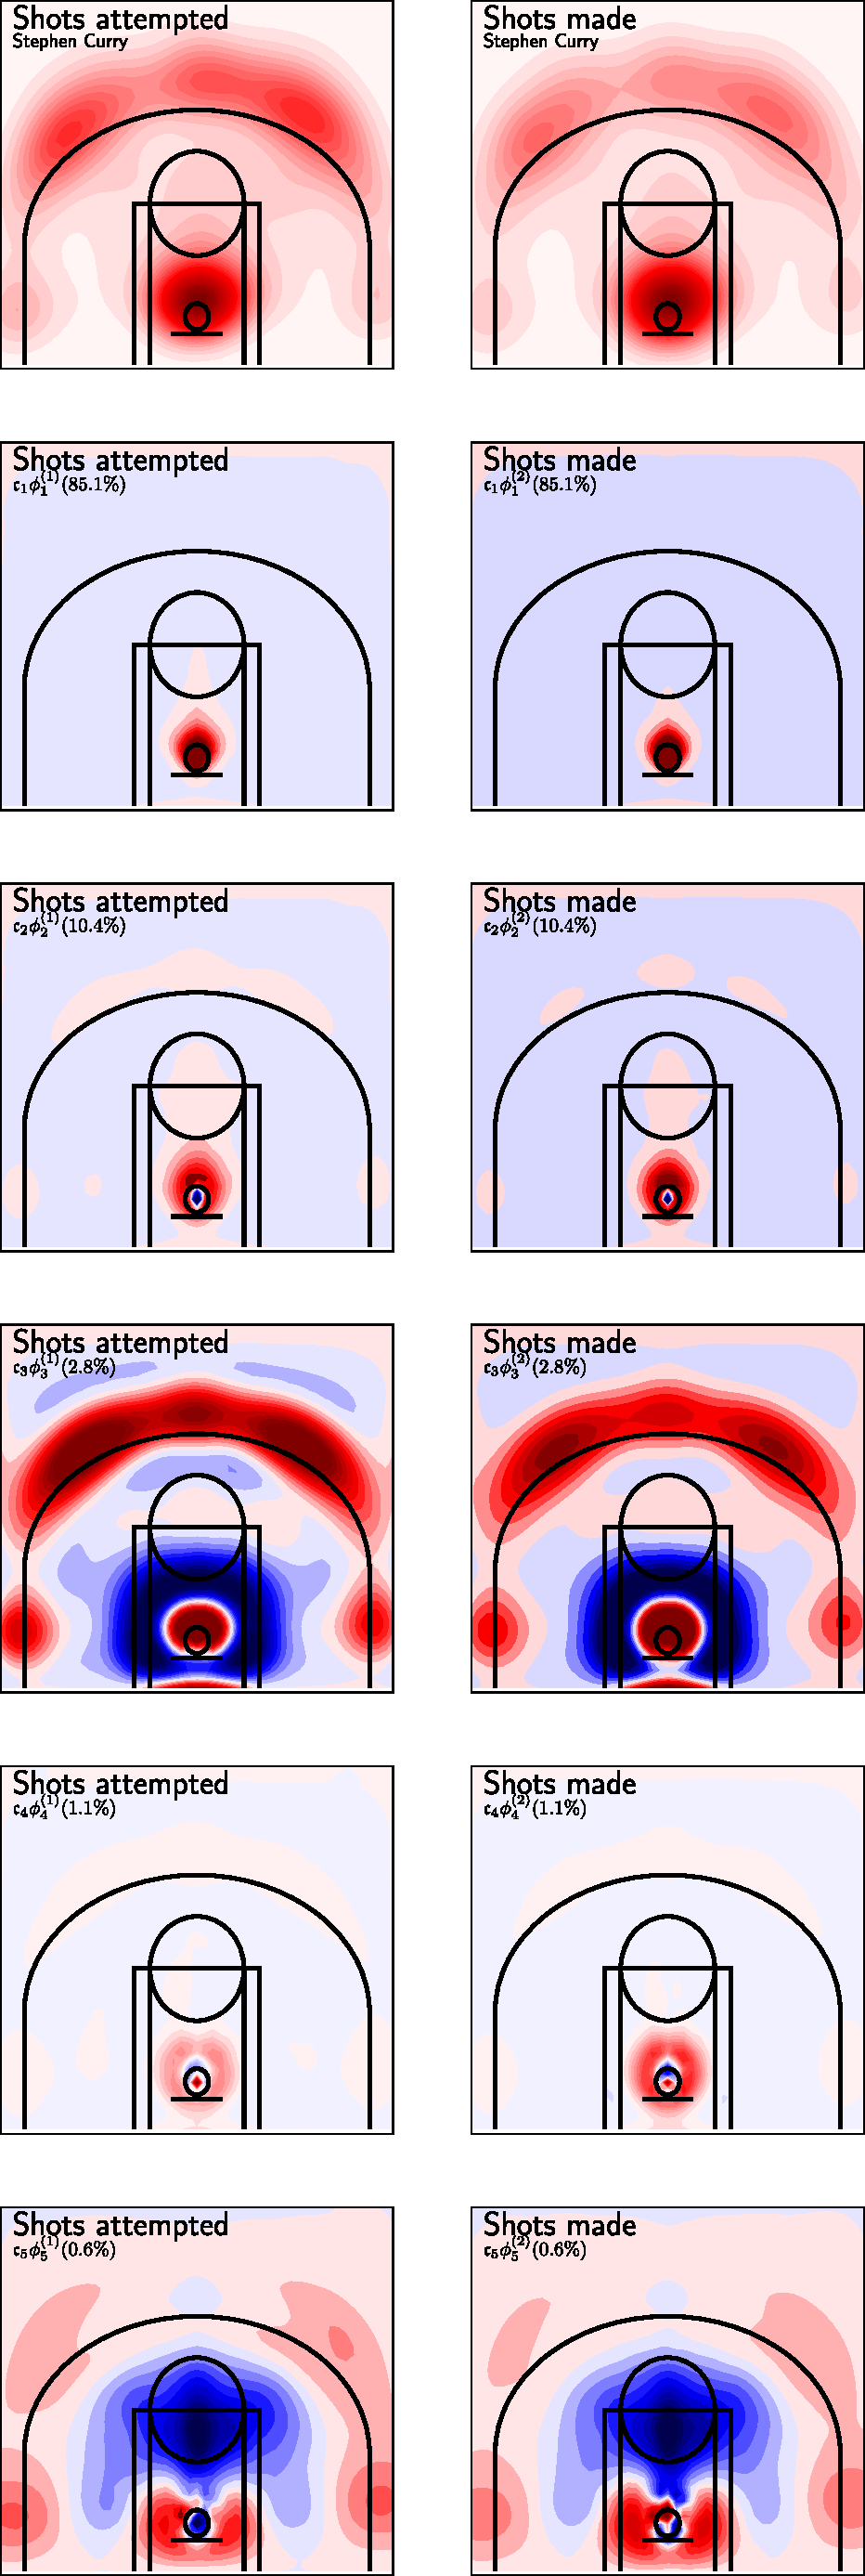
\includegraphics[width=\textwidth]{figures/curry_decomposition.pdf}
        \caption{Gram matrix}
        \label{fig:curry_decomposition}
    \end{subfigure}
    \hfill
    \begin{subfigure}[b]{0.45\textwidth}
        \centering
        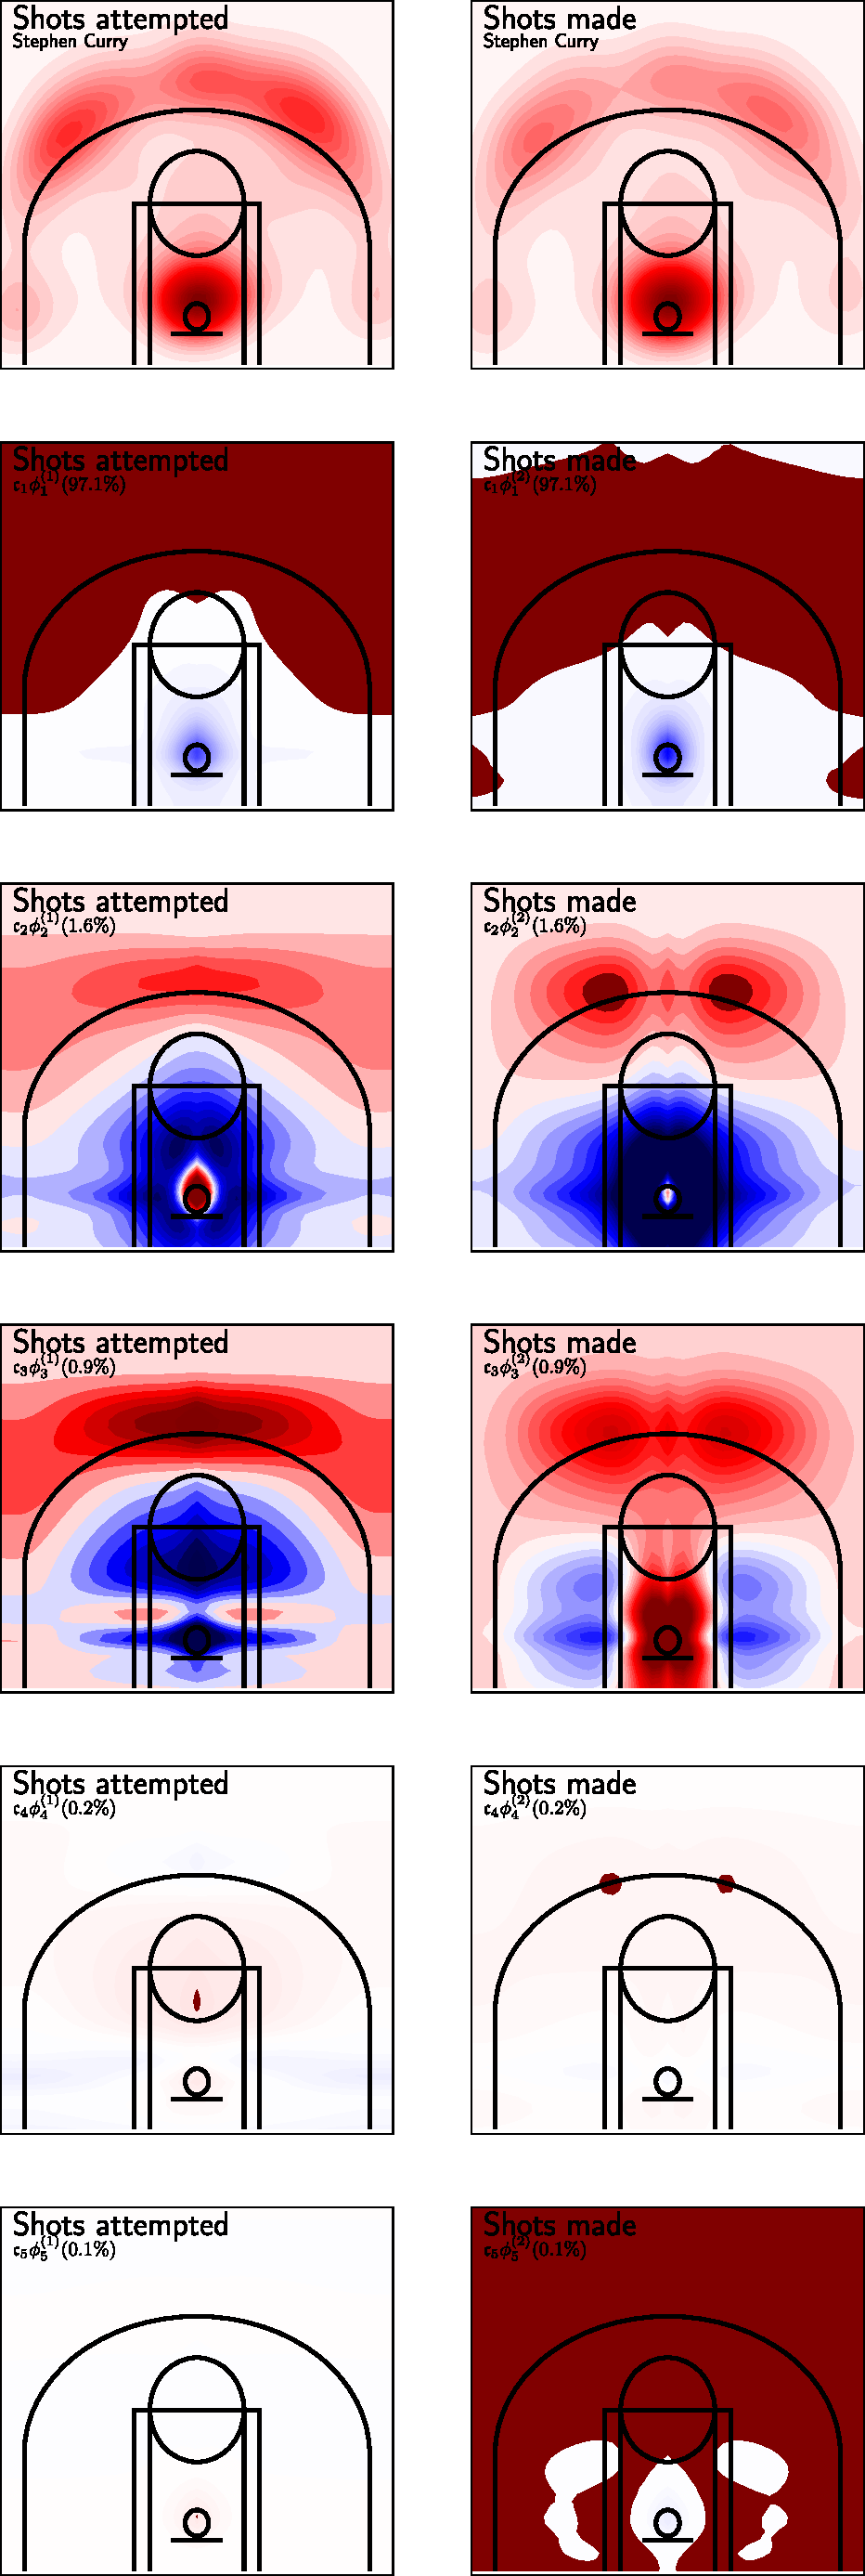
\includegraphics[width=\textwidth]{figures/curry_decomposition_fcptpa.pdf}
        \caption{FCPTPA}
        \label{fig:curry_decomposition_fcptpa}
    \end{subfigure}
    \caption{Decomposition for Stephen Curry.}
    \label{fig:curry_shoots_decomposition}
\end{figure}

% section application (end)